%%% LaTeX Template: Article/Thesis/etc. with colored headings and special fonts
%%%
%%% Source: http://www.howtotex.com/
%%% Feel free to distribute this template, but please keep to referal to http://www.howtotex.com/ here.
%%% February 2011
%%%
%%% Last updated September 2018 by CDM

%%%  Preamble
\documentclass[11pt,letterpaper]{article}
\usepackage[margin=1.0in]{geometry}
\usepackage[T1]{fontenc}
\usepackage[bitstream-charter]{mathdesign}
\usepackage[latin1]{inputenc}					
\usepackage{amsmath}						
\usepackage{xcolor}
\usepackage{cite}
\usepackage{hyphenat}
\usepackage{graphicx}
\usepackage{float}
\usepackage{subfigure}
\usepackage{sectsty}
\usepackage[compact]{titlesec} 
\usepackage[tablegrid]{vhistory}
\allsectionsfont{\color{accentcolor}\scshape\selectfont}

%%% Definitions
\definecolor{accentcolor}{rgb}{0.0,0.0,0.5} 
\newcommand{\teamname}{Senior Rangers}
\newcommand{\productname}{Voice Print}
\newcommand{\coursename}{CSE 4316: Senior Design I}
\newcommand{\semester}{Fall 2018}
\newcommand{\docname}{Project Charter}
\newcommand{\department}{Department of Computer Science \& Engineering}
\newcommand{\university}{The University of Texas at Arlington}
\newcommand{\authors}{Brian Leonard \\ Kamal Mistry \\ Quy Pham \\ Peter Severynen \\ William Wallace \\}

%%% Headers and footers
\usepackage{fancyhdr}
	\pagestyle{fancy}						% Enabling the custom headers/footers
\usepackage{lastpage}	
	% Header (empty)
	\lhead{}
	\chead{}
	\rhead{}
	% Footer
	\lfoot{\footnotesize \teamname \ - \semester}
	\cfoot{}
	\rfoot{\footnotesize page \thepage\ of \pageref{LastPage}}	% "Page 1 of 2"
	\renewcommand{\headrulewidth}{0.0pt}
	\renewcommand{\footrulewidth}{0.4pt}

%%% Change the abstract environment
\usepackage[runin]{abstract}			% runin option for a run-in title
%\setlength\absleftindent{30pt}			% left margin
%\setlength\absrightindent{30pt}		% right margin
\abslabeldelim{\quad}	
\setlength{\abstitleskip}{-10pt}
\renewcommand{\abstractname}{}
\renewcommand{\abstracttextfont}{\color{accentcolor} \small \slshape}	% slanted text

%%% Start of the document
\begin{document}

%%% Cover sheet
{\centering \huge \color{accentcolor} \sc \textbf{\department \\ \university} \par}
\vspace{1 in}
{\centering \huge \color{accentcolor} \sc \textbf{\docname \\ \coursename \\ \semester} \par}
\vspace{0.5 in}
\begin{figure}[h!]
	\centering
   	
\includegraphics[width=0.40\textwidth]{images/charter_img}
\end{figure}
\vspace{0.5 in}
{\centering \huge \color{accentcolor} \sc \textbf{\teamname \\ \productname} \par}
\vspace{0.5 in}
{\centering \large \sc \textbf{\authors} \par}
\newpage


%\vspace{1 in}
%\centerline{January 13th, 2012}
%\newpage

%%% Revision History
\begin{versionhistory}
  	\vhEntry{0.1}{9.23.2018}{B.L., P.S., K.M., Q.P., W.W.}{document creation}
  	\vhEntry{1.0}{10.01.2018}{B.L., P.S., K.M., Q.P., W.W.}{Release candidate}
\end{versionhistory}
\newpage

%%% Table of contents
\tableofcontents
\newpage

%%% List of figures and tables (optional)
%\listoffigures
%\listoftables
%\newpage
\setcounter{table}{0}

%%% Agile project charter sections
\section{Vision}
The vision defines the "Why" of the project. This is the higher purpose, or the reason for the project’s existence. This section should avoid mentioning implementation details, and focus more on what the current problem is and what would be gained if the problem were to be solved. 

\section{Mission}
This is the "What" of the project and it states what will be done in the project to achieve its higher purpose (the higher purpose being the vision” discussed above). This section should focus mostly on what your solution is going to be and what it is going to do.
\section{Success Criteria}
VoicePrint will be successful if we have:
\begin{itemize}
\end{itemize}
\begin{itemize}
\item 25,000 total downloads after 6 months
\item 50,000 total downloads after 12 months
\item 100,000 downloads after 24 months
\end{itemize}


\newpage

%%% Remaining project charter sections
\section{Background}
The inspiration for \textit{VoicePrint} began long ago. One of its creators grew up watching \textit{Star Trek: The Next Generation}. On this television program, there is a device called the Replicator. When users speak to the ship's computer, the Replicator executes their commands and creates the three-dimensional object that they requested. During the summer of 2018, this team member decided to make a simpler version of the Replicator in real-life. It would be a smartphone app that would take speech input from the user, send commands to a 3D printer, and print 3D objects. This developer watched YouTube videos about 3D printing and voice commands, and he built Android apps in Java.

In the fall, a team formed around this idea. Our team has four computer science majors. Our diverse team combines experience with mobile app development, Java programming, and software engineering, with seven years of project management experience in industry. \textit{VoicePrint} has been approved, and the work has begun in earnest.
\section{Related Work}
There are a few options for voice-activated printers on the market now.
\begin{itemize}
  \item HP announced a general platform for their printers earlier in 2018 that uses the Google Cloud and Amazon Alexa and enables functionality such as asking "Am I low on blank ink?" Or specifying "Print three copies" \cite{HP2018}.
  \item Xerox AltaLink devices utilize IBM's Watson technology to skip input screens and icons and perform tasks such as scanning, emailing, and initiating service requests through voice commands \cite{Xerox2018}.
\end{itemize}
These solutions are only designed for traditional printers, and are not suitable for printing 3D objects.
\begin{itemize}
  \item Yahoo Japan has developed a voice-activated 3D printer for visually-impaired children \cite{Yahoo2013}.
\end{itemize}
This implementation is only intended for simple shapes and is not suitable for complex 3D printing.
\begin{itemize}
  \item XYZprinting has a feature on it's Da Vinci Color AiO 3D printer to receive certain voice commands \cite{XYZ2018}.
\end{itemize}
This product is more expensive than would be feasible for most end users, and the voice commands are limited to simple instructions.
\newpage\section{System Overview}
This project contains 4 big block components:
\begin{itemize}
 
\item Controller 

\item Google Cloud Speech API

\item OctoPrint

\item 3D Printer

\end{itemize}

Function of each component:

\begin{itemize}

\item Controller: Takes speech and .STL file as input.

\item Google Cloud Speech API: receives speech from user, then converts speech to text. 

In the other words, Google Cloud Speech API works as a audio transcription.

\item OctoPrint: interface to adjust setting on the printer and to print object.

\item 3D Printer: print 3D object from user's commands.

\end{itemize}

\begin{figure}[h!]
	\centering
   	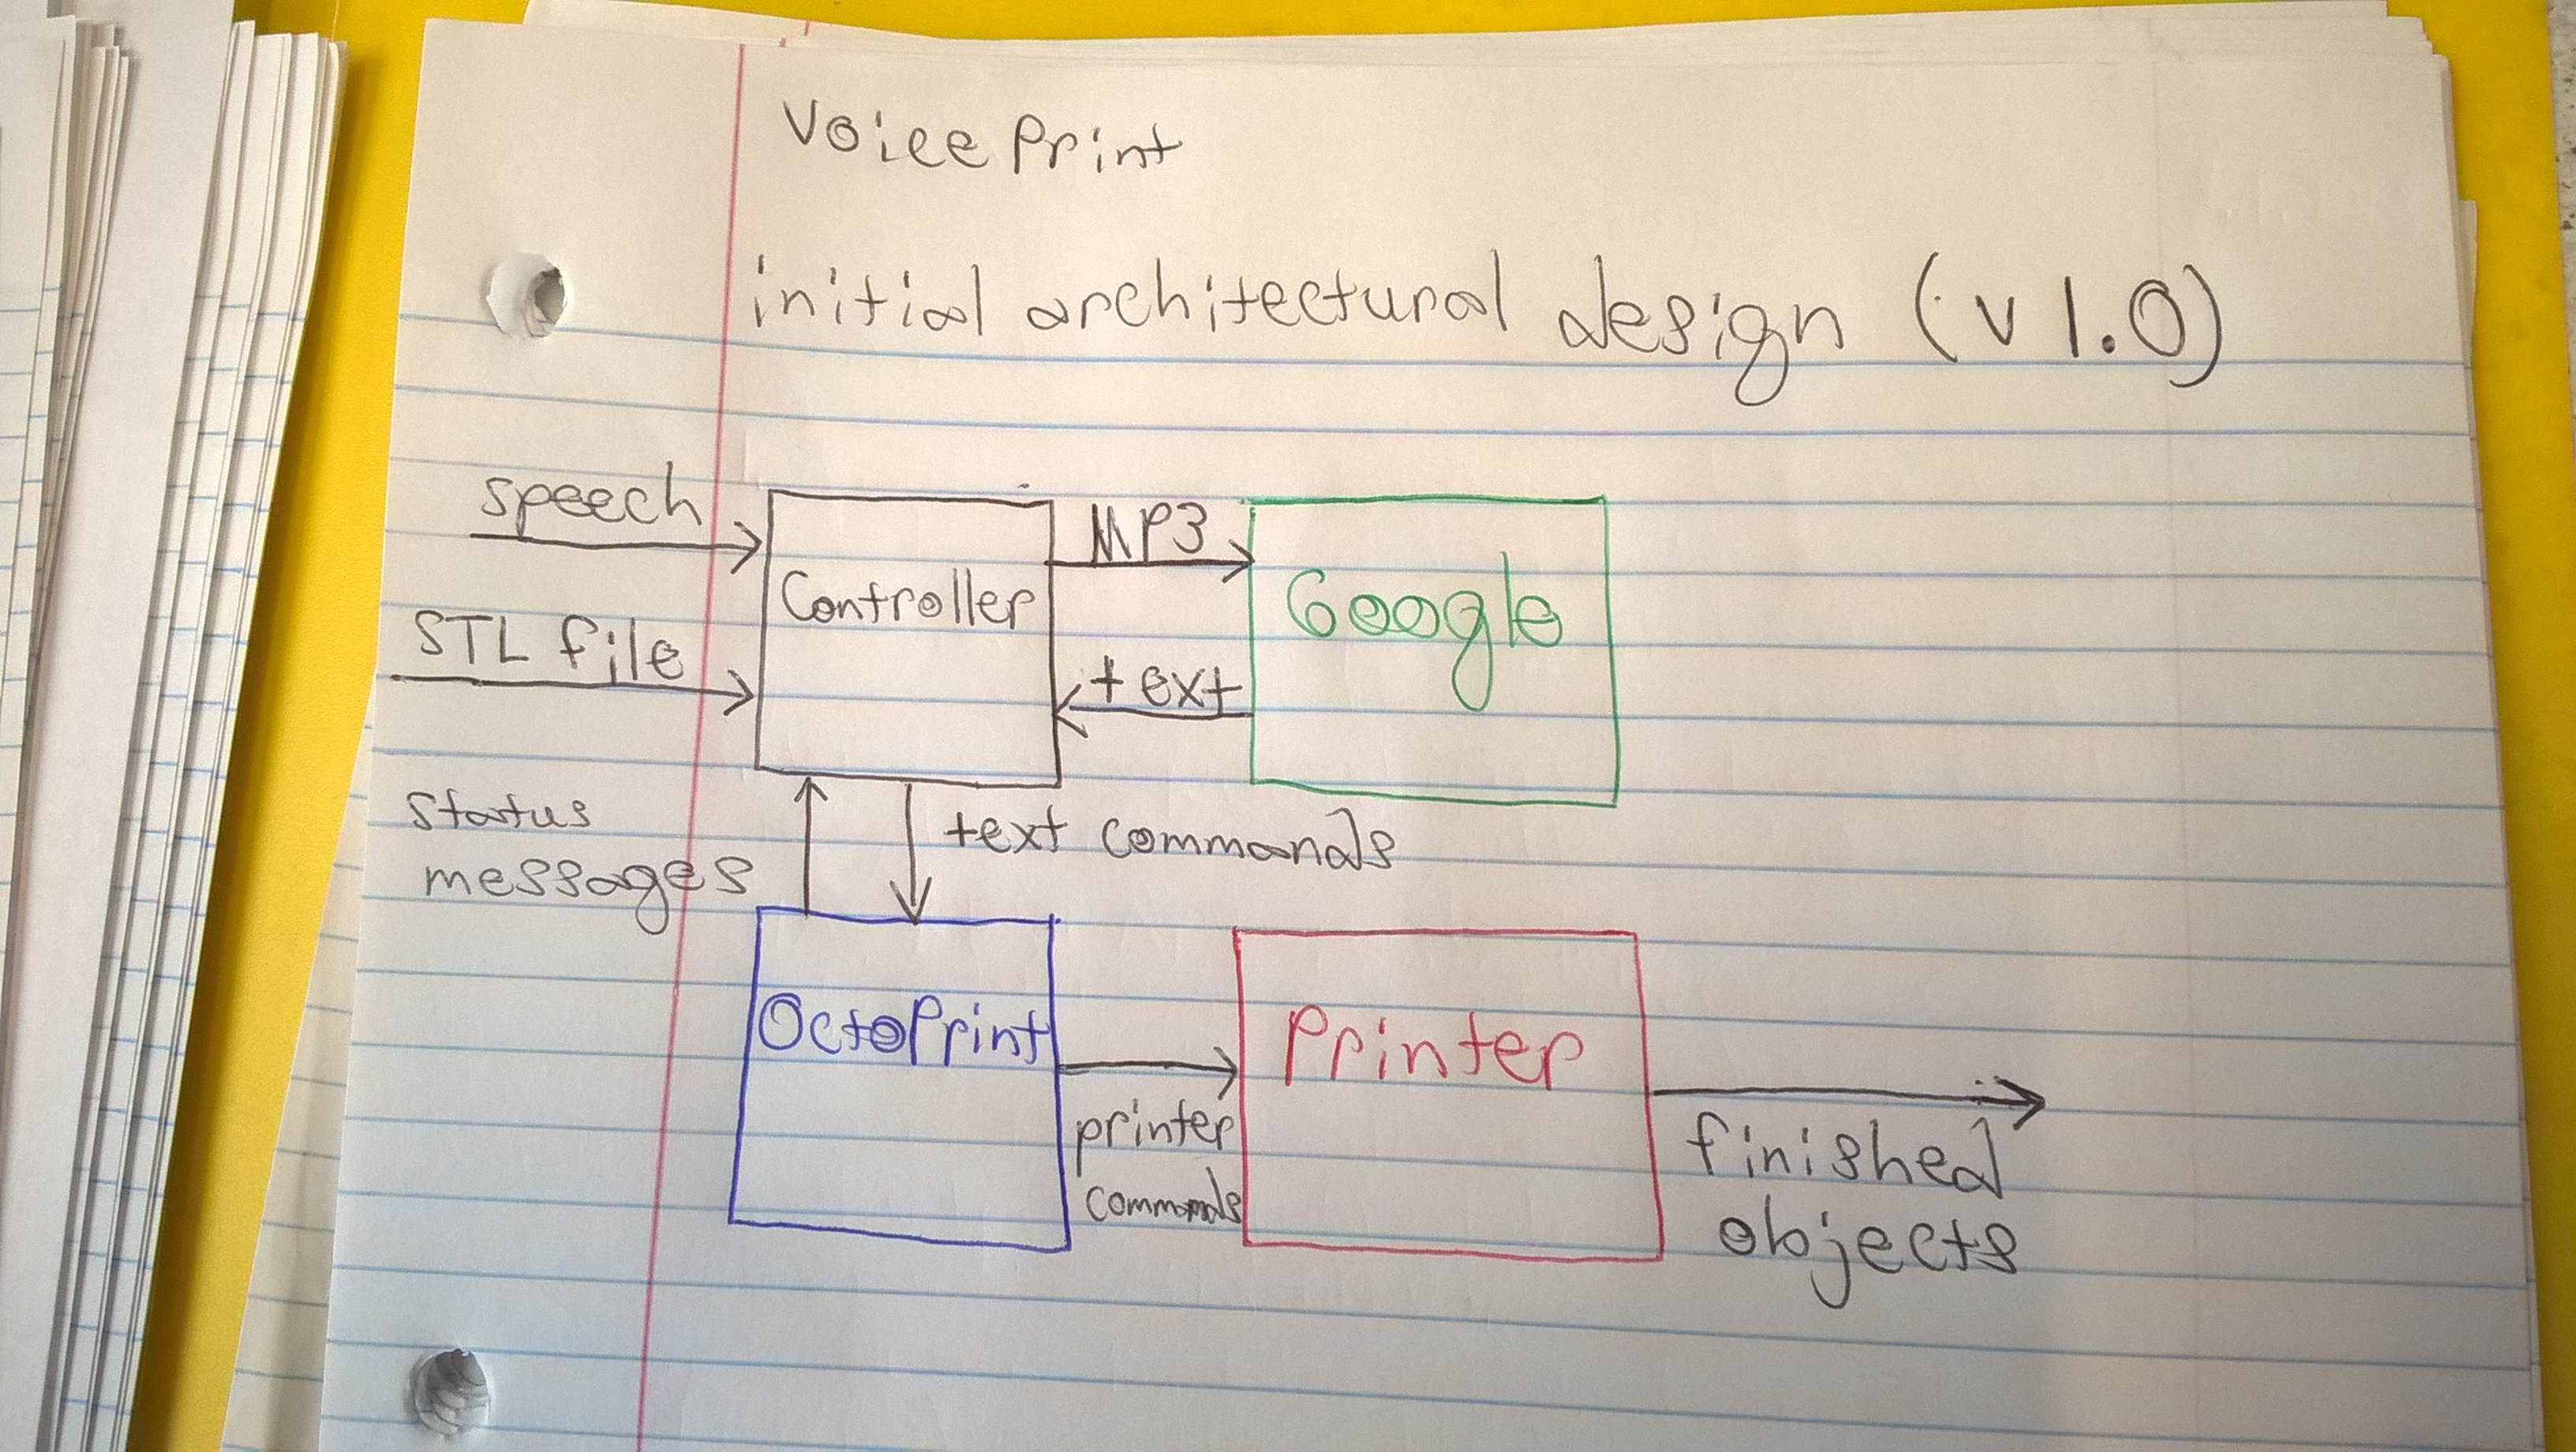
\includegraphics[width=0.6\textwidth]{images/Diagram.jpg}
   	    \caption{Diagram of major components of VoicePrint}

\end{figure}



\newpage\section{Roles \& Responsibilities}
The primary stakeholders of the VoicePrint project are the end users who will use this software to print physical objects. Additional stakeholders are the development team members creating the application. The supervising professor, Dr. Christopher D. McMurrough, is also a stakeholder. There is no sponsor or immediate customer. The development team consists of five members:
\begin{itemize}
    \item Brian Leonard
    \item Kamal Mistry
    \item Quy Pham
    \item Peter Severynen
    \item William Wallace
\end{itemize}
Every member of the team is in the Computer Science Engineering field, and each will assist with the actual programming. The additional roles will start as follows:
\begin{itemize}
  \item Product Owner: Peter Severynen
  \item Scrum Master: Brian Leonard
\end{itemize}
The Product Owner role will remain with Peter, as the project was originally his idea. This allows a single point of escalation with regards to design decisions, which removes development obstacles before they arise.
The Scrum Master role will rotate with each sprint. Brian has previous project management experience and will take charge of the first sprint, and each member will have a turn in later iterations.
\section{Cost Proposal}
\subsection{Cost Proposal}
\textit{VoicePrint} is an android application which will be developed by integrating multiple softwares and hardwares as below.
\\
Support will be provided by department of CSE. Below is the list of major expenses towards the project.
\\
1. Google Cloud Speech-to-text API for translations (software)
\\
2. Amazon Alexa to support voice commands (hardware)
\\
3. Octoprint software which supports 3D printers for functions (software)
\\
4. An android phone to test the application on (hardware)
\\
5. Ultimaker filaments to 3D printers (Materials)

\subsection{Preliminary Budget}
\begin{tabular}{|l|c|r|}
	\hline
    Components or Tools & Units & Price\\
    \hline
    \hline
	Speech-to-Text API & NA & \$0.006 per 15 seconds\\
	\hline
	Amazon Alexa (Echo Plus) & 1 & \$179.99\\
	\hline
	Octoprint & 1 & Opensource\\
	\hline
	Android (jellybeans 5.5) & 1 & \$120.00\\
	\hline
	Filaments & 750g & \$49.99\\
	\hline
\end{tabular}

\subsection{Current \& Pending Support}
We only have a funding source which is the department of CSE. They are providing the fund of \$800 the maximum. \\
\section{Facilities \& Equipment}
Since this project is more software-oriented, neither lab space nor a testing ground is required. However, we will need to borrow a 3D printer in the senior design lab for testing. The Raspberry Pi connected to the 3D printer will also be used to interface with the printer using OctoPrint. We will also need to purchase filament in order to use the 3D printers and print objects from our app. Additional equipment may include Alexa, Amazon's voice assistant, and Google Home. This equipment will be used only if we decide to implement these services in our app. Finally, to test our app we will need an Android phone running Jellybean 5.5 or later. Anything that is not present in the lab but is required for the project will be purchased using our given budget from the CSE department. 
\section{Assumptions}
An assumption is a belief of what you assume to be true in the future. You make assumptions based on your knowledge, experience or the information available on hand. These are anticipated events or circumstances that are expected to occur during your project's life cycle.

Assumptions are supposed to be true but do not necessarily end up being true. Sometimes they may turn out to be false, which can affect your project significantly. They add risks to the project because they may or may not be true. For example, if you are working on an outdoor unmanned vehicle, are you assuming that testing space will be available when needed? Are you relying on an external team or contractor to provide a certain subsystem on time? If you are working at a customer facility or deploying on their computing infrastructure, are you assuming you will be granted physical access or network credentials?

This section should contain a list of at least 5 of the most critical assumptions related to your project. For example:

The following list contains critical assumptions related to the implementation and testing of the project.

\begin{itemize}
  \item A suitable outdoor testing location will be available by the 3rd sprint cycle
  \item The X sensing system developed by Sensor Consulting Company will be delivered according to specifications by the 4th sprint cycle
  \item Access to the customer installation site will be provided by the 5th sprint cycle
  \item The customer will provide ample power and network connectivity at the installation site
  \item The installation site network infrastructure will allow TCP network traffic on port 8080
\end{itemize}
\section{Constraints}
The following list contains key constraints related to the development and usage of \textit{VoicePrint}:

\begin{itemize}
  \item Final prototype demonstration must be completed by May 1st, 2019
  \item The 3D printers at the Senior Design Lab are only available for testing during normal business hours
  \item Total development costs must not exceed \$800
  \item All app development will be completed by team members
  \item 
\end{itemize}
\newpage\section{Risks}
This section should contain a list of at least 5 of the most critical risks related to your project. Additionally, the probability of occurrence, size of loss, and risk exposure should be listed. For size of loss, express units as the number of days by which the project schedule would be delayed. For risk exposure, multiply the size of loss by the probability of occurrence to obtain the exposure in days. For example:

The following high-level risk census contains identified project risks with the highest exposure. Mitigation strategies will be discussed in future planning sessions.

\begin{table}[h]
\resizebox{\textwidth}{!}{
\begin{tabular}{|l|l|l|l|}
\hline
 \textbf{Risk description} & \textbf{Probability} & \textbf{Loss (days)} & \textbf{Exposure (days)} \\ \hline
 Availability of X sensor module due to contractor delay  & 0.50 & 20 & 10 \\ \hline
 Outdoor testing grounds are not available  & 0.20 & 14 & 2.8 \\ \hline
 Internet access not available at installation site  & 0.30 & 9 & 2.7 \\ \hline
 Delays in shipping from overseas vendors  & 0.10 & 20 & 2.0 \\ \hline
 Certification delays at compliance testing facility & 0.15 & 10 & 1.5 \\ \hline
\end{tabular}}
\caption{Overview of highest exposure project risks} 
\end{table}
\section{Documentation \& Reporting}
%%% In this section, you will describe all of the various artifacts that you will generate and maintain during the project life cycle. Describe the purpose of each item below, how the content will be generated, where it will be stored, how often it will be updated, etc. Replace the default text for each section with your own description. Reword this paragraph as appropriate.

\subsection{Major Documentation Deliverables}

\subsubsection{Project Charter}
This document will be updated every sprint to reflect any changes the project may encounter. The changes may include: additional equipment/expenditures, added/removed functionality, etc. The initial version of this charter will be delivered Monday, October 1st and the final version will be delivered at the end of Senior Design II along with the final product.

\subsubsection{System Requirements Specification}
The system requirements specification will be be completed by the end of the second sprint on October 23rd. Any changes will be approved by team agreement, and the final version will be turned in along with the final product.

\subsubsection{Architectural Design Specification}
The architectural design specification document will be updated any time the team agrees that it needs to be changed. Any member may propose changes via Slack, and the team will discuss whether the change is appropriate and required. The Product Owner will be the final authority on changes to this document. The initial version will be completed by the end of Sprint \#3, on November 13th, and the final version will be part of the completed project.

\subsubsection{Detailed Design Specification}
The detailed design specification will be updated with each sprint, to match the reality of the project. This document will be completed next semester, exact dates not yet finalized.

\subsection{Recurring Sprint Items}

\subsubsection{Product Backlog}
Items from the SRS will be added to the product backlog based on how the overall architecture of the app is laid out. For example, requirements dealing with the interfaces to the OctoPrint and Google Cloud Speech APIs would be some of the first items to be added to the product backlog. These decisions will be decided by a team vote and the product backlog will be maintained/shared as an Excel spreadsheet on the team's Google Drive.

\subsubsection{Sprint Planning}
In each sprint, the whole team will meet for approximately one hour per week to plan the next sprint. In this meeting, they will agree to complete a number of items from the product backlog during the next sprint. Based on the results of this meeting, a sprint backlog will be defined for the next sprint. The sprint backlog will be incorporated into the sprint plan. The project will consist of 8 sprints (4 sprints in Senior Design I and 4 sprints in Senior Design II).

\subsubsection{Sprint Goal}
The development team will decide the sprint goal for each sprint by majority vote with the advice of the scrum master. Based on the customer's requirements, the Product Owner will list the objectives that the sprint should achieve. Then, the development team will select items from the product backlog that help meet the sprint goal. 

\subsubsection{Sprint Backlog}
The development team will decide which product backlog items are incorporated into the sprint backlog for each sprint. The sprint backlog will be maintained/shared as an Excel spreadsheet on the team's Google Drive. 

\subsubsection{Task Breakdown}
Individual tasks from the sprint backlog may be assigned in one of two ways: 
\begin{itemize}

\item If the tasks are of equal difficulty, as determined by the Scrum Master, then any team member may voluntarily claim that task.

\item If some tasks are more difficult than others, as determined by the Scrum Master, then a team member may claim them if and only if he is technically competent in that area or has demonstrated a willingness to learn how to perform that task. 

\item If the Scrum Master decides that a task is too large for one team member to complete within the allotted time, then he will divide it into multiple sub tasks and these will be assigned as stated above. Optionally, two team members may elect to work together on the task. 

\end{itemize}
Depending on the end date of each sprint, team members will estimate the time that they think they will need to complete their tasks. Note: Each member's estimated task completion date must be earlier than the end date. 

\subsubsection{Sprint Burn Down Charts}
For each sprint, team members will keep updating the "Status" column for their assigned tasks. As long as the "Status" column is updated to "Finished", the sprint burn down chart will be updated and generated automatically. 

The total amount of effort expended by each individual team member may be accessed as follows:

\begin{itemize}
    
\item In a sprint backlog spreadsheet, click on the "Assigned to" column to see the tasks that have been assigned to each member and click on the "Status" column to see which of these tasks have been completed. 

\end{itemize}
The sprint burn down chart will be formatted as a release burn down chart.
An example of a sprint burn down chart chart is shown in Figure 2 on the next page.

\begin{figure}[h!]
	\centering
   	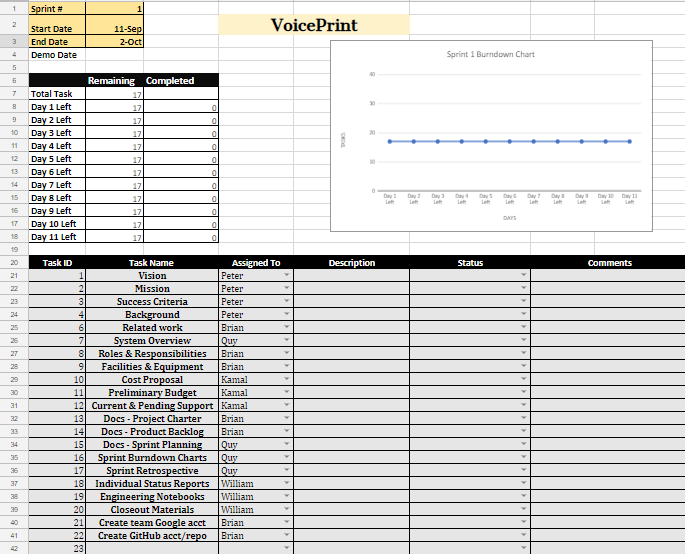
\includegraphics[width=0.6\textwidth]{images/Chart.png}
    \caption{Example sprint burn down chart}
\end{figure}

\newpage\subsubsection{Sprint Retrospective}
For each sprint, the team will schedule a sprint review and a sprint retrospective. The time and date of these meetings will be decided by a majority vote of the team members on Slack. During the sprint review, the development team will discuss the items from the product backlog that they completed during the sprint. In the sprint retrospective, the team will discuss the process characteristics in which they performed satisfactorily and the areas in which they need to improve. The whole team will participate in these meetings/presentations. All tasks must be completed at least 3 days before the due day of the sprint.

\subsubsection{Individual Status Reports}
For each sprint, each team member will submit an individual status report. This report will show that individual's status on a given sprint (behind, ahead, etc). Some key items included in the status report include: the sprint goal, backlog, logged hours, burn down chart, and individual retrospective.

\subsubsection{Engineering Notebooks}
Each team member must add at least one page to his engineering notebook each week. To maintain accountability, the team will meet before and/or after class every Monday and Wednesday. Each page shall be signed by a witness. Any team member may serve as a witness and sign any other team member's notebook.

\subsection{Closeout Materials}

\subsubsection{System Prototype}
The \textit{VoicePrint} system prototype will be an operational app installable to Android devices that allows a user to print a 3D object using voice commands. It will be demonstrated in the CSE Senior Design Lab.

\subsubsection{Project Poster}
The project poster will be 3' x 3' and will include information about 3D printing in general, how \textit{VoicePrint} works, and will have pictures of the application and at least one finished object printed by voice commands.

\subsubsection{Web Page}
The project web page will include a walkthrough of the application's functionality. Each option will be explained and a tutorial will be available to help new users utilize the app. Source code documentation will be included on one page.

\subsubsection{Demo Video}
The demo video will show how the app works. The video will show step-by-step how the app operates, beginning from the setup and ending with a finished 3D printed object. The video will be at most 5 minutes.

\subsubsection{Source Code}
\textit{VoicePrint} source code will be maintained on GitHub, which provides version control as well. No source will be provided to end users.  Inside the application will be an "about" option that lists any relevant licenses used.

\subsubsection{Source Code Documentation}
Doxygen will be used for source code documentation. The final documentation will be exported to the web page.

\subsubsection{Installation Scripts}
Installation will be performed by simply installing the final .apk to an end user's Android device. No additional considerations for servers should be necessary, as the only external communication required will be handled by API calls to Google or Amazon.

\subsubsection{User Manual}
A user manual will be provided in the app displayed as a help button. Setup as well as instructions on how to operate the app will be located here.

\newpage

%%% References
\bibliographystyle{plain}
\bibliographystyle{reference/IEEEtran_custom}
\bibliography{reference/refs}{}

\end{document}